\chapter{System Architecture and Development} \label{sec:systemdevelopment}

In the previous chapter I presented the requirements the solution had to achieve and evaluated different development options, discussing their advantages and disadvantages.
I closed the chapter with a solution proposition, where I justified hardware and software choices.
In this chapter I will present the implementation of such solution, going through the architecture design, configuration and development. 

\section{Architecture}

The architecture identically follows the EPCGlobal example, presented in figure~\ref{fig:archstructure} on chapter~\ref{sec:epcglobal}.
A detailed overview of the architecture is illustrated in figure~\ref{fig:practicalarchitecture}.

\begin{figure}
    \centering
    \caption{Overview of the solution architecture developed in this dissertation} 
    \label{fig:practicalarchitecture}
\end{figure}

The Impinj Speedway R120 reader and Keonn Advantenna-p14 are attached behind the bottom shelf, as shown in figure~\ref{fig:shelvephoto}, radiating the entire shelve.
The reader interrogates the tags, using the \ac{gen2} Tag Air Standard, following the active \acp{rospec} configured prior to the inventory.
The inventory information is sent inside \texttt{RO\_ACCESS\_REPORT} messages, to the \ac{llrp} interface of the middleware.

\begin{figure}
    \centering
    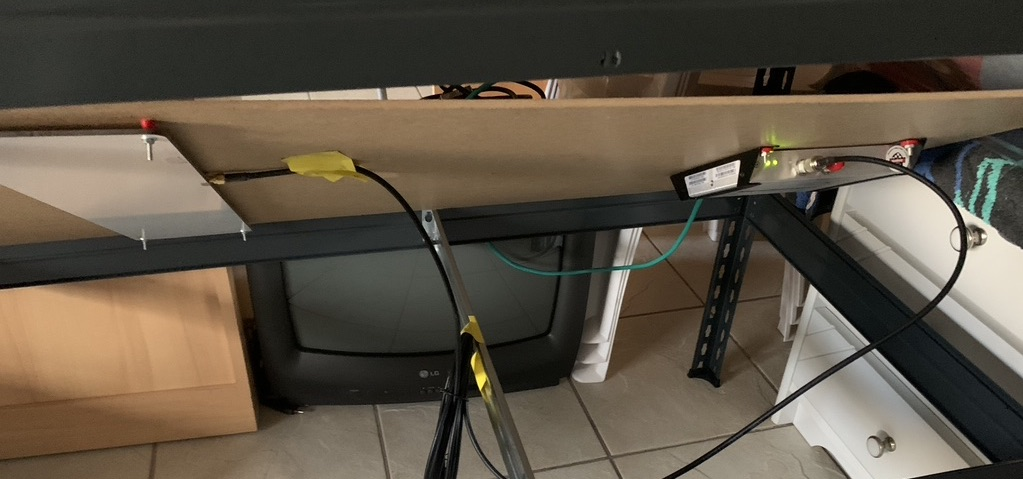
\includegraphics[width=\textwidth]{figs/completeshelve_photo.jpeg}
    \caption{Photograph of the Keonn Advantenna-p14 and Impinj Speedway R120 attached behind the bottom shelf}
    \label{fig:shelvephoto}
\end{figure}

The Fosstrak \ac{fc} middlware receives the inventory information from the reader, processes it, following the configured \acp{ecspec}, and periodically generates \acp{ecreport}, which are sent to the capture application \ac{ale} capture interface.

The Fosstrak capture application receives the \acp{ecreport}, contextualizes them and runs additional business logic. The contextualized data is aggregated in \acs{epcis} documents, following the \ac{cbv} vocabulary guidelines, and sent to the \ac{epcis} repository.

The \ac{epcis} repository permanently saves the \ac{epcis} data in to the \ac{epcis} database. The \ac{epcis} repository exposes the \ac{soap} query interface, which can be used to retrieve information.

The managing application to visualize the smart shelve inventory, was made using web technologies. The application is served to browsers, which query the data from the \ac{epcis} repository.
Modern browsers do not support \ac{soap} natively. 
To mitigate this problem, the requests pass through a crude \ac{epcis} web adapter, serving as a proxy between web applications and the \ac{epcis} repository. 
The proxy adapts the \ac{soap} \ac{xml} requests into \ac{http} and \ac{json} endpoints, which modern browsers understand.

All requests hitting the platform go through an NGINX reverse proxy. This hides the topology and characteristics of the back-end servers, removing the direct internet access to them. The services on the platform are kept inside a non-public subnet and concentrate the access control on that single point. The NGINX server also allows load balancing between the services, which is useful when there is a need to scale the platform. The proxy also deals with cross-origin resource sharing mechanism, freeing the servers from dealing with it.

\section{\acs{epc} Serialization Plan}

When companies adhere to the EPCGlobal framework, there are a few things they have to deliberate.
One of those is delineating the \acs{epc} serialization plan, where an evaluation of unique products and serial numbers is made.
The plan has to ensure that a company has enough unique product numbers to identify current and future products.

In the case of this dissertation, the serialization plan was already performed by Nespresso.
Each of their products has already an assigned \ac{gtin}, including the cardboard case for transport.

From the product cases and sleeves, used for testing, Nespresso has two company prefixes registered, 

\section{Reader}

Update ao firmware do leitor. origen 5.12.2.240 (Build cbc9ad1d0d1)

%ver https://support.impinj.com/hc/en-us/articles/360000046899-Reader-Modes-Made-Easy
%ver Reader and Gateway compatibility: %https://support.impinj.com/hc/en-us/articles/360000046899-Reader-Modes-Made-Easy
%quote https://support.impinj.com/hc/en-us/articles/360007414920-Reader-Mode-1002-Autoset-Dense-Reader-Deep-Scan-Overview

Octane 6.2.0 is based on \ac{llrp} version 1.0.1, which does not support C1G2 version 1.2.0.~\cite[sec. 3.1.21]{ImpinjOctaneLLRP}. Octane includes vendor extensions to expose the underlying air protocol features. For more information, refer to the documentation for the individual extensions.

\paragraph{ROBoundarySpec}

This parameter carries the lifetime of the Reader inventory and survey operation.
ROSpecStartTrigger, ROSpecStopTrigger: This is the start and stop trigger for this ROSpec.

Used ROSpecStopTriggerType Periodic.
Periodic trigger values: period - Time period specified in milliseconds; offset - Time offset specified in milliseconds from receiving message to start. useful for one-shot inventory.

Used ROSpecStartTriggerType Periodic.

\paragraph{Antenna inventory operations configuration (\ac{aispec})}

AISpecStopTrigger parameter defines the stop (i.e., terminating boundary) of an antenna inventory operation~\cite[sec. 11.2.2.1]{LowLevelReader}. Here it was set to Null to Stop when \ac{rospec} is done.

InventoryParameterSpec Configuration (C1G2InventoryCommand) \dots

RF transmitter: Power, hoptableid, channelindex \dots

TagInventoryStateAware flag is used to determine how to process all the C1G2Filter and C1G2Singulation parameters in this command. At a functional level, if the Client is managing the tag states during an inventory operation (i.e., the Client is specifying Class1 Gen2 tag Select command Target and Action values), then it will set that flag to true and pass the appropriate fields in the C1G2 Filter and C1G2 Singulation parameters. If a reader set CanDoTagInventoryStateAwareSingulation to False in LLRPCapabilities (section 10.2.2), then the Reader SHALL ignore the TagInventoryStateAware flag.

The C1G2RFControl parameter~\cite[sec. 3.1.4]{ImpinjOctaneLLRP} specifies Speedway Gen2 modes selected by Impinj system engineering to provide the best performance. No Tari adjustment is necessary. Tari values passed by the client will be ignored.

Mode Index for the use case in this dissertation can be one of the three bellow, depending on the RF environment in which is deployed: 

\begin{itemize}
    \item (the choice) 1002 (Autoset Static) configures the Reader to choose the best Gen2 link parameters for the environments where the tags population is relatively static and we wish to attempt to search for the weakest tag.
    \item 1003 (Autoset Static Fast) is an adaptation of Autoset Static for good RF environments
    \item 1004 (Autoset Static DRM) is an adaptation of Autoset Static for difficult RF environments
\end{itemize}

This C1G2SingulationControl Parameter provides controls particular to the singulation process in the C1G2 air protocol.

\begin{itemize}
    \item Tag transit time: This is the measure of expected tag mobility in the field of view of the antenna where this inventory operation is getting executed.
    \item Tag population: This is the expected tag population in the field of view of the antenna.
    \item Session ID: This is the C1G2 session number that the tags use to update the inventory state upon successful singulation.
    \item  TagInventoryStateAwareSingulationAction: This is not used since the TagInventoryStateAware flag is set to false in the InventoryParameterSpec.
\end{itemize}

This parameters were not set to let the Impinj mode index use the optimal parameters.

\paragraph{Report Operation Report Spec (ROReportSpec)}

Describes the messages and parameters used in reports, event notifications and keepalives that are generated by the Reader and sent to the Client.

A reporting trigger (ROReportTrigger or AccessReportTrigger) generates a report while a connection is open.

In the use case in this dissertation we are not concerned with near real-time updates on the state of the inventory. So we can reduce the report generation by letting the end of the ROSpec generate a report periodically.
So ROReportTrigger can be set to \texttt{Upon\_N\_Tags\_Or\_End\_Of\_ROSpec} with N=0 (unlimited tag in antenna's field of view)~\cite[sec. 14.2.1]{LowLevelReader}

In terms of the content useful to retrieve from the reader inventory singulation, the ROSpecID, FirstSeenTimestamp, LastSeenTimestamp are in the interests of the application.

We can enable it the TagReportContentSelector block by setting the Enable in each on.

\paragraph{Impinj Custom Parameters}

Impinj readers support Impinj extensions to the \ac{llrp} protocol. This extensions can be disabled by setting their values to zero. This will use the information defined in the \ac{llrp} parameters defined above.

One that is worth looking at is the ImpinjInventorySearchMode.
Impinj Readers implement state unaware singulation and therefore the Client does not control how the Reader attempts to singulate tags. This parameter provides a high-level control over the search algorithm and consequently does not interfere with any of the standard \ac{llrp} settings.~\cite[sec. 4.3.3]{ImpinjOctaneLLRP}

Value 3, Single Target Inventory with Suppression (aka TagFocus), used for High tag count, high-throughput use cases where a reduction in repeated tag observations is acceptable. Suppresses repeated observations for extended periods of time while tags are energized. Supported only with Monza tags using Session 1. Since the we are using Monza R6-P tags, we can enable this mode.

\paragraph{Tools}

Used Fosstrak \ac{llrp} Commander with the old old Eclipse 3.3 and JRE/JDK 1.8 to configure de reader using an xml schema.
Also developed a java tool to configure the reader using \ac{llrp}. Used the java llrp. LTK and code by impinj to configure it based on the "same" schema used in the LLRP commander.
In the java tool, the xml parser sometimes requires fields that shouldn't be needed because Impinj reader ignores then in certain configuration options. But for the configuration to be validated, they have to be present in order to validate de xsd schema (TagInventoryStateAware, Tari)

\section{Middleware}

\paragraph{LRSpec}

\paragraph{ECSpec}

We have 2 ec reports: one for informing the tag uri added and deleted from the shelve that will be used for the capture application to provide supply chain visualization to the epcis repository; a second for informing the real-time inventory service on the point of sale the current state of inventory (will sent counts for products).

ECSpec2: want only to know the number of which coffee type are available in storage, so SGTIN filter value of 1 (Point of Sale (POS) Trade Item), with nespresso's company prefix, different item references groups and any serial tag number in those groups.

%Table 10-1 in sec 10.2 TDS : Filter Values for SGTIN EPC Tags
%Ref ECReportOutputSpec in 8.2.10 ALE standard core

\section{Capture application}

\section{EPCIS repository}

\section{Managements application}